\newcommand{\pluseq}{\mathrel{+}=}

In this section, we describe the learning algorithm that we used to maximize the number of purchases made by users that have reached our website by clicking on ads.

\subsubsection{Assumptions}
\begin{enumerate}
    \item There is only one phase
    \item The allocation of the budget over the three subcampaigns is fixed
\end{enumerate}

\subsubsection{Setup of the experiment}
3 Thompson Sampling learners are used, one for each class of users. Since the users arrive on the purchase page by clicking on the ads, we assume that we can differentiate them by their class, thus proposing a different price to each user.

To satisfy assumption (1), the algorithm runs for a limited number of days, 45, enough to provide a significant result.

The average number of users that arrive per day are taken from the results of the previous point, which optimizes the budget in the fourth phase and maximizes the number of clicks. It returns the following average number of daily clicks: $C=[1800, 12000, 350]$. For this experiment, we will use these values as the daily average number of clicks, with a variance that is proportional to each value: $Var_i = C_i / 4$ $\forall{i} \in \{1,2,3\}$.

Since the optimization of the budget is made once a day and depends on the price chosen, also the price (for each class of users) is chosen once per day.

The minimum and maximum prices (0, 400) are the same for all the classes of users. The same goes for the number of arms, for which we tested various configurations ranging from 4 to 10 arms to see which one provided the best result.

\subsubsection{The algorithm}
The high-level pseudo code of the algorithm is shown in Algorithm \ref{alg:ts_pricing}.

Each TS learner is responsible for a class of users. Each day, the 3 learners pull the best price from their beta distributions. The prices are then proposed to all the users that arrive to the website on that day after clicking on the ads. At the end of the day, the learners are updated with the number of successes (purchases) for each class.

\begin{algorithm}
    \caption{TS learners for pricing}
    \label{alg:ts_pricing}
	\begin{algorithmic}[1]
        \STATE $J\gets ${ all classes of users}
        \STATE $T\gets ${ 45 days }
        \STATE $regret\gets ${0}
        \FOR{$day \in T $}
		\FOR{$j \in \{1,...,J\}$}
		\STATE $price\gets ${Draw a price from the j-th TS learner}
        \STATE $successes\gets ${number of buys with pulled price}
        \STATE $failures\gets ${clicks[j][day] - successes}
        \STATE $reward\gets ${successes * price}
        \STATE regret += optimum - reward
        \STATE TS[j].update(pulledArm, successes, failures)
        \ENDFOR
        \ENDFOR
	\end{algorithmic}
\end{algorithm}

Some remarks:
\begin{itemize}
    \item on line 6, to draw a price means that for each arm $a$ we pull a sample $\theta_a$ from the beta distributions, and then return the price $p_a$ of the arm that offers the best reward, that is $p_a = \underset{p_a}{argmax} \{p_a * \theta_a\}$
    \item on line 11 the update of the TS learner consists in updating the beta parameters of the arm pulled $\bar{a}$, in the following way: $(\alpha, \beta)_{\bar{a}} \pluseq (successes, failures)$
\end{itemize}

\subsubsection{Choice of the best arm}
The following results come from averaging over 1000 experiments.

We tested the experiment with several numbers of arms. For each number $n$ of arms, draw the $n$ prices equally spaced in the interval and run the experiment, calculate the regret and the reward and use them to choose the best number of arms.

\makebox[\textwidth][c]{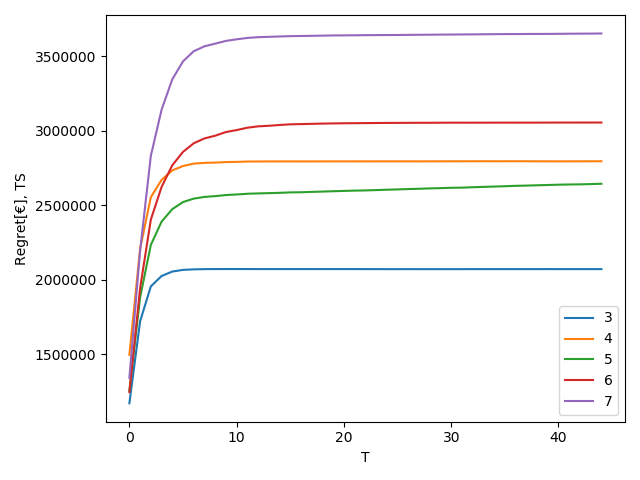
\includegraphics[width=0.85\textwidth]{sections/images/pricing_regret.png}}

The first image shows the cumulative regret using different numbers of arms, ranging from 3 to 7.
Given the limited time-span, the best result is provided by a low number of arms, which converges more rapidly to the best arm.

However, since in the calculus of the regret we use as clairvoyant the best possible arm, we know how fast the learner converges but not how much money we would be losing in the ideal case in which we could use an infinite number of arms. For this reason, we set up another experiment in which we calculate the reward and compare it with the clairvoyant reward that, in this case, corresponds with the reward that we would get if we chose, for each class, its actual best price.

\makebox[\textwidth][c]{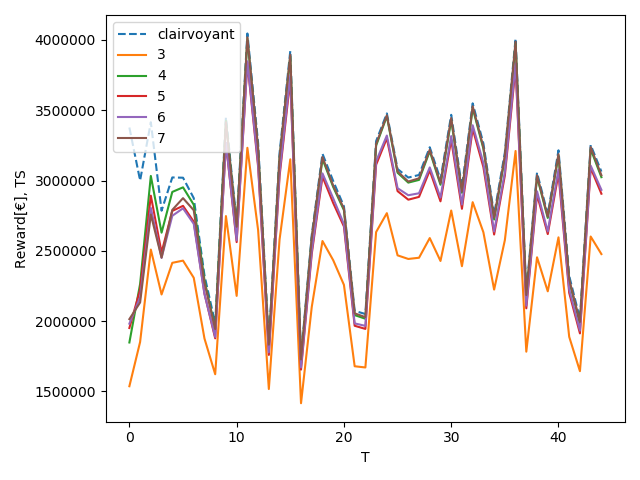
\includegraphics[width=0.85\textwidth]{sections/images/pricing_reward.png}}
\makebox[\textwidth][c]{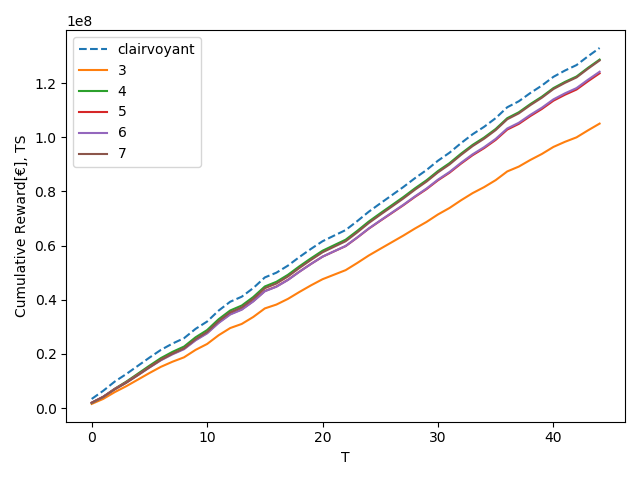
\includegraphics[width=0.85\textwidth]{sections/images/pricing_cumulative_reward.png}}
As the image shows, using 3 arms does not offer a good reward. The best number of arms that comes out from our experiment is 4, which is aligned with the theoretical expection that we have with a period of 45 days.

\subsubsection{Results}
With 4 arms, we have a reasonably fast convergence to the best arm and enough arms to pull a price that is close enough to the clairvoyant to obtain a good reward.